% Options for packages loaded elsewhere
\PassOptionsToPackage{unicode}{hyperref}
\PassOptionsToPackage{hyphens}{url}
\PassOptionsToPackage{dvipsnames,svgnames,x11names}{xcolor}
%
\documentclass[
  letterpaper,
  DIV=11,
  numbers=noendperiod]{scrreprt}

\usepackage{amsmath,amssymb}
\usepackage{iftex}
\ifPDFTeX
  \usepackage[T1]{fontenc}
  \usepackage[utf8]{inputenc}
  \usepackage{textcomp} % provide euro and other symbols
\else % if luatex or xetex
  \usepackage{unicode-math}
  \defaultfontfeatures{Scale=MatchLowercase}
  \defaultfontfeatures[\rmfamily]{Ligatures=TeX,Scale=1}
\fi
\usepackage{lmodern}
\ifPDFTeX\else  
    % xetex/luatex font selection
\fi
% Use upquote if available, for straight quotes in verbatim environments
\IfFileExists{upquote.sty}{\usepackage{upquote}}{}
\IfFileExists{microtype.sty}{% use microtype if available
  \usepackage[]{microtype}
  \UseMicrotypeSet[protrusion]{basicmath} % disable protrusion for tt fonts
}{}
\makeatletter
\@ifundefined{KOMAClassName}{% if non-KOMA class
  \IfFileExists{parskip.sty}{%
    \usepackage{parskip}
  }{% else
    \setlength{\parindent}{0pt}
    \setlength{\parskip}{6pt plus 2pt minus 1pt}}
}{% if KOMA class
  \KOMAoptions{parskip=half}}
\makeatother
\usepackage{xcolor}
\setlength{\emergencystretch}{3em} % prevent overfull lines
\setcounter{secnumdepth}{5}
% Make \paragraph and \subparagraph free-standing
\makeatletter
\ifx\paragraph\undefined\else
  \let\oldparagraph\paragraph
  \renewcommand{\paragraph}{
    \@ifstar
      \xxxParagraphStar
      \xxxParagraphNoStar
  }
  \newcommand{\xxxParagraphStar}[1]{\oldparagraph*{#1}\mbox{}}
  \newcommand{\xxxParagraphNoStar}[1]{\oldparagraph{#1}\mbox{}}
\fi
\ifx\subparagraph\undefined\else
  \let\oldsubparagraph\subparagraph
  \renewcommand{\subparagraph}{
    \@ifstar
      \xxxSubParagraphStar
      \xxxSubParagraphNoStar
  }
  \newcommand{\xxxSubParagraphStar}[1]{\oldsubparagraph*{#1}\mbox{}}
  \newcommand{\xxxSubParagraphNoStar}[1]{\oldsubparagraph{#1}\mbox{}}
\fi
\makeatother

\usepackage{color}
\usepackage{fancyvrb}
\newcommand{\VerbBar}{|}
\newcommand{\VERB}{\Verb[commandchars=\\\{\}]}
\DefineVerbatimEnvironment{Highlighting}{Verbatim}{commandchars=\\\{\}}
% Add ',fontsize=\small' for more characters per line
\usepackage{framed}
\definecolor{shadecolor}{RGB}{241,243,245}
\newenvironment{Shaded}{\begin{snugshade}}{\end{snugshade}}
\newcommand{\AlertTok}[1]{\textcolor[rgb]{0.68,0.00,0.00}{#1}}
\newcommand{\AnnotationTok}[1]{\textcolor[rgb]{0.37,0.37,0.37}{#1}}
\newcommand{\AttributeTok}[1]{\textcolor[rgb]{0.40,0.45,0.13}{#1}}
\newcommand{\BaseNTok}[1]{\textcolor[rgb]{0.68,0.00,0.00}{#1}}
\newcommand{\BuiltInTok}[1]{\textcolor[rgb]{0.00,0.23,0.31}{#1}}
\newcommand{\CharTok}[1]{\textcolor[rgb]{0.13,0.47,0.30}{#1}}
\newcommand{\CommentTok}[1]{\textcolor[rgb]{0.37,0.37,0.37}{#1}}
\newcommand{\CommentVarTok}[1]{\textcolor[rgb]{0.37,0.37,0.37}{\textit{#1}}}
\newcommand{\ConstantTok}[1]{\textcolor[rgb]{0.56,0.35,0.01}{#1}}
\newcommand{\ControlFlowTok}[1]{\textcolor[rgb]{0.00,0.23,0.31}{\textbf{#1}}}
\newcommand{\DataTypeTok}[1]{\textcolor[rgb]{0.68,0.00,0.00}{#1}}
\newcommand{\DecValTok}[1]{\textcolor[rgb]{0.68,0.00,0.00}{#1}}
\newcommand{\DocumentationTok}[1]{\textcolor[rgb]{0.37,0.37,0.37}{\textit{#1}}}
\newcommand{\ErrorTok}[1]{\textcolor[rgb]{0.68,0.00,0.00}{#1}}
\newcommand{\ExtensionTok}[1]{\textcolor[rgb]{0.00,0.23,0.31}{#1}}
\newcommand{\FloatTok}[1]{\textcolor[rgb]{0.68,0.00,0.00}{#1}}
\newcommand{\FunctionTok}[1]{\textcolor[rgb]{0.28,0.35,0.67}{#1}}
\newcommand{\ImportTok}[1]{\textcolor[rgb]{0.00,0.46,0.62}{#1}}
\newcommand{\InformationTok}[1]{\textcolor[rgb]{0.37,0.37,0.37}{#1}}
\newcommand{\KeywordTok}[1]{\textcolor[rgb]{0.00,0.23,0.31}{\textbf{#1}}}
\newcommand{\NormalTok}[1]{\textcolor[rgb]{0.00,0.23,0.31}{#1}}
\newcommand{\OperatorTok}[1]{\textcolor[rgb]{0.37,0.37,0.37}{#1}}
\newcommand{\OtherTok}[1]{\textcolor[rgb]{0.00,0.23,0.31}{#1}}
\newcommand{\PreprocessorTok}[1]{\textcolor[rgb]{0.68,0.00,0.00}{#1}}
\newcommand{\RegionMarkerTok}[1]{\textcolor[rgb]{0.00,0.23,0.31}{#1}}
\newcommand{\SpecialCharTok}[1]{\textcolor[rgb]{0.37,0.37,0.37}{#1}}
\newcommand{\SpecialStringTok}[1]{\textcolor[rgb]{0.13,0.47,0.30}{#1}}
\newcommand{\StringTok}[1]{\textcolor[rgb]{0.13,0.47,0.30}{#1}}
\newcommand{\VariableTok}[1]{\textcolor[rgb]{0.07,0.07,0.07}{#1}}
\newcommand{\VerbatimStringTok}[1]{\textcolor[rgb]{0.13,0.47,0.30}{#1}}
\newcommand{\WarningTok}[1]{\textcolor[rgb]{0.37,0.37,0.37}{\textit{#1}}}

\providecommand{\tightlist}{%
  \setlength{\itemsep}{0pt}\setlength{\parskip}{0pt}}\usepackage{longtable,booktabs,array}
\usepackage{calc} % for calculating minipage widths
% Correct order of tables after \paragraph or \subparagraph
\usepackage{etoolbox}
\makeatletter
\patchcmd\longtable{\par}{\if@noskipsec\mbox{}\fi\par}{}{}
\makeatother
% Allow footnotes in longtable head/foot
\IfFileExists{footnotehyper.sty}{\usepackage{footnotehyper}}{\usepackage{footnote}}
\makesavenoteenv{longtable}
\usepackage{graphicx}
\makeatletter
\newsavebox\pandoc@box
\newcommand*\pandocbounded[1]{% scales image to fit in text height/width
  \sbox\pandoc@box{#1}%
  \Gscale@div\@tempa{\textheight}{\dimexpr\ht\pandoc@box+\dp\pandoc@box\relax}%
  \Gscale@div\@tempb{\linewidth}{\wd\pandoc@box}%
  \ifdim\@tempb\p@<\@tempa\p@\let\@tempa\@tempb\fi% select the smaller of both
  \ifdim\@tempa\p@<\p@\scalebox{\@tempa}{\usebox\pandoc@box}%
  \else\usebox{\pandoc@box}%
  \fi%
}
% Set default figure placement to htbp
\def\fps@figure{htbp}
\makeatother
% definitions for citeproc citations
\NewDocumentCommand\citeproctext{}{}
\NewDocumentCommand\citeproc{mm}{%
  \begingroup\def\citeproctext{#2}\cite{#1}\endgroup}
\makeatletter
 % allow citations to break across lines
 \let\@cite@ofmt\@firstofone
 % avoid brackets around text for \cite:
 \def\@biblabel#1{}
 \def\@cite#1#2{{#1\if@tempswa , #2\fi}}
\makeatother
\newlength{\cslhangindent}
\setlength{\cslhangindent}{1.5em}
\newlength{\csllabelwidth}
\setlength{\csllabelwidth}{3em}
\newenvironment{CSLReferences}[2] % #1 hanging-indent, #2 entry-spacing
 {\begin{list}{}{%
  \setlength{\itemindent}{0pt}
  \setlength{\leftmargin}{0pt}
  \setlength{\parsep}{0pt}
  % turn on hanging indent if param 1 is 1
  \ifodd #1
   \setlength{\leftmargin}{\cslhangindent}
   \setlength{\itemindent}{-1\cslhangindent}
  \fi
  % set entry spacing
  \setlength{\itemsep}{#2\baselineskip}}}
 {\end{list}}
\usepackage{calc}
\newcommand{\CSLBlock}[1]{\hfill\break\parbox[t]{\linewidth}{\strut\ignorespaces#1\strut}}
\newcommand{\CSLLeftMargin}[1]{\parbox[t]{\csllabelwidth}{\strut#1\strut}}
\newcommand{\CSLRightInline}[1]{\parbox[t]{\linewidth - \csllabelwidth}{\strut#1\strut}}
\newcommand{\CSLIndent}[1]{\hspace{\cslhangindent}#1}

\KOMAoption{captions}{tableheading}
\makeatletter
\@ifpackageloaded{bookmark}{}{\usepackage{bookmark}}
\makeatother
\makeatletter
\@ifpackageloaded{caption}{}{\usepackage{caption}}
\AtBeginDocument{%
\ifdefined\contentsname
  \renewcommand*\contentsname{Table of contents}
\else
  \newcommand\contentsname{Table of contents}
\fi
\ifdefined\listfigurename
  \renewcommand*\listfigurename{List of Figures}
\else
  \newcommand\listfigurename{List of Figures}
\fi
\ifdefined\listtablename
  \renewcommand*\listtablename{List of Tables}
\else
  \newcommand\listtablename{List of Tables}
\fi
\ifdefined\figurename
  \renewcommand*\figurename{Figure}
\else
  \newcommand\figurename{Figure}
\fi
\ifdefined\tablename
  \renewcommand*\tablename{Table}
\else
  \newcommand\tablename{Table}
\fi
}
\@ifpackageloaded{float}{}{\usepackage{float}}
\floatstyle{ruled}
\@ifundefined{c@chapter}{\newfloat{codelisting}{h}{lop}}{\newfloat{codelisting}{h}{lop}[chapter]}
\floatname{codelisting}{Listing}
\newcommand*\listoflistings{\listof{codelisting}{List of Listings}}
\makeatother
\makeatletter
\makeatother
\makeatletter
\@ifpackageloaded{caption}{}{\usepackage{caption}}
\@ifpackageloaded{subcaption}{}{\usepackage{subcaption}}
\makeatother

\usepackage{bookmark}

\IfFileExists{xurl.sty}{\usepackage{xurl}}{} % add URL line breaks if available
\urlstyle{same} % disable monospaced font for URLs
\hypersetup{
  pdftitle={Mass Spec Academy},
  colorlinks=true,
  linkcolor={blue},
  filecolor={Maroon},
  citecolor={Blue},
  urlcolor={Blue},
  pdfcreator={LaTeX via pandoc}}


\title{Mass Spec Academy}
\author{}
\date{}

\begin{document}
\maketitle

\renewcommand*\contentsname{Table of contents}
{
\hypersetup{linkcolor=}
\setcounter{tocdepth}{2}
\tableofcontents
}

\bookmarksetup{startatroot}

\chapter{Mass Spec Academy}\label{mass-spec-academy}

\begin{figure}[H]

{\centering 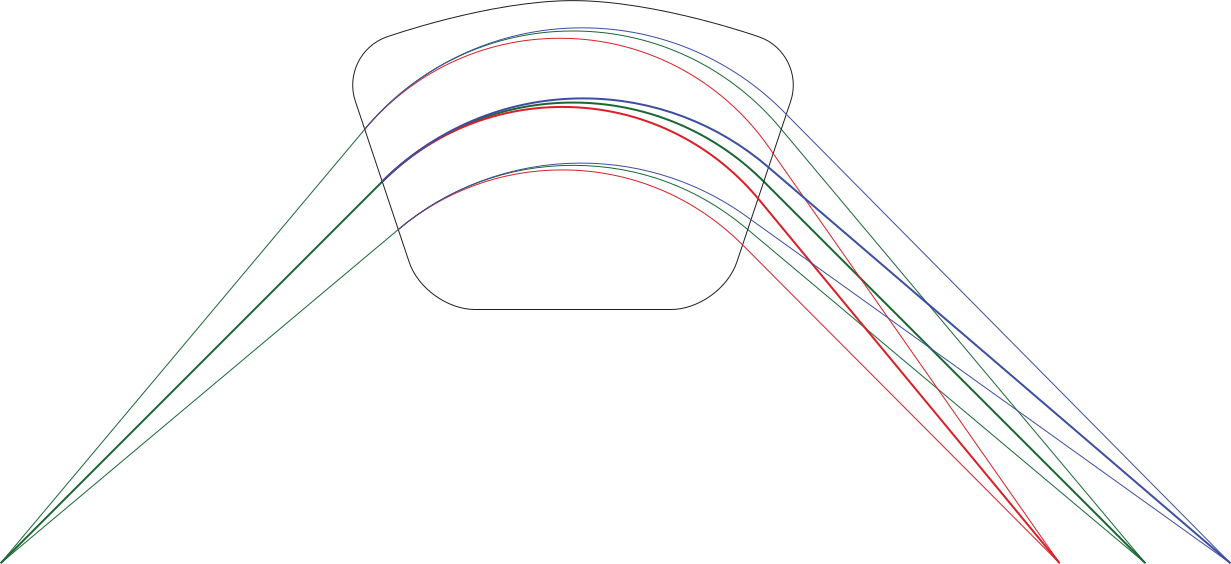
\includegraphics[width=0.6\linewidth,height=\textheight,keepaspectratio]{index_files/mediabag/figs/ExtendedGeometryLineDrawing.pdf}

}

\caption{Magnetic Sector with Extended Geometry}

\end{figure}%

\bookmarksetup{startatroot}

\chapter{Project Description}\label{project-description}

The goal of this project is to create an online resource that provides
comprehensive and accessible information on mass spectrometry methods
used in geochronology, comprising:

\begin{itemize}
\tightlist
\item
  A detailed description and history of the method
\item
  Best practices for sample preparation and analysis
\item
  A guide to data and uncertainty analysis
\item
  Applications, and case studies from peer-reviewed research
\item
  Short exercises and worked solutions appropriate for graduate
  students.
\end{itemize}

\subsection{Funding}\label{funding}

\emph{This material is based upon work supported by the National Science
Foundation under Grant Nos. EAR-2218547 and -2218544. Any opinions,
findings, and conclusions or recommendations expressed in this material
are those of the author(s) and do not necessarily reflect the views of
the National Science Foundation. Thanks to the AGeS program for its
support.}

\begin{figure}

\begin{minipage}{0.25\linewidth}
~\end{minipage}%
%
\begin{minipage}{0.25\linewidth}
\pandocbounded{\includegraphics[keepaspectratio]{figs/AGeS_logo_0.jpg}}\end{minipage}%
%
\begin{minipage}{0.25\linewidth}
\pandocbounded{
\includegraphics[keepaspectratio]{index_files/mediabag/figs/NSF_Official_logo_CMYK.pdf}}\end{minipage}%
%
\begin{minipage}{0.25\linewidth}
~\end{minipage}%

\end{figure}%

\bookmarksetup{startatroot}

\chapter{Physics and Chemistry
Refresher}\label{physics-and-chemistry-refresher}

\section{Background: Basic Concepts}\label{background-basic-concepts}

\subsection{Forget the Spectrometer, What is a
Mass?}\label{forget-the-spectrometer-what-is-a-mass}

\subsubsection{SI units for mass}\label{si-units-for-mass}

The SI unit for mass is the kilogram, but samples analyzed for mass
spectrometry are usually much smaller. The table below lists some
typical sample sizes for geochemistry, both as SI terms with prefixes
and as fractions of a gram. As we will soon learn, the number of atoms
in a gram depends on the atomic mass of the atoms. The third column
gives the number of atoms of that mass. It starts with atoms of mass 12
unified mass units (i.e., \(^{12}\)C), but you can hover your slider
over the blue atomic mass and drag left or right to increase or decrease
its value.

\begin{longtable}[]{@{}
  >{\raggedright\arraybackslash}p{(\linewidth - 6\tabcolsep) * \real{0.2368}}
  >{\raggedright\arraybackslash}p{(\linewidth - 6\tabcolsep) * \real{0.2368}}
  >{\raggedright\arraybackslash}p{(\linewidth - 6\tabcolsep) * \real{0.2632}}
  >{\raggedright\arraybackslash}p{(\linewidth - 6\tabcolsep) * \real{0.2632}}@{}}
\caption{SI prefixes for small things.}\tabularnewline
\toprule\noalign{}
\begin{minipage}[b]{\linewidth}\raggedright
Mass with Prefix
\end{minipage} & \begin{minipage}[b]{\linewidth}\raggedright
Mass in grams
\end{minipage} & \begin{minipage}[b]{\linewidth}\raggedright
Atoms of \(^{12}\)C
\end{minipage} & \begin{minipage}[b]{\linewidth}\raggedright
Atoms of \(^{238}\)U
\end{minipage} \\
\midrule\noalign{}
\endfirsthead
\toprule\noalign{}
\begin{minipage}[b]{\linewidth}\raggedright
Mass with Prefix
\end{minipage} & \begin{minipage}[b]{\linewidth}\raggedright
Mass in grams
\end{minipage} & \begin{minipage}[b]{\linewidth}\raggedright
Atoms of \(^{12}\)C
\end{minipage} & \begin{minipage}[b]{\linewidth}\raggedright
Atoms of \(^{238}\)U
\end{minipage} \\
\midrule\noalign{}
\endhead
\bottomrule\noalign{}
\endlastfoot
kilogram & \(10^3\) grams & \(6 \times 10^{26}\) &
\(3 \times 10^{25}\) \\
gram & 1 gram & \(6 \times 10^{23}\) & \(3 \times 10^{22}\) \\
miligram & \(10^{-3}\) grams & \(6 \times 10^{20}\) &
\(3 \times 10^{19}\) \\
microgram & \(10^{-6}\) grams & \(6 \times 10^{17}\) &
\(3 \times 10^{16}\) \\
nanogram & \(10^{-9}\) grams & \(6 \times 10^{14}\) &
\(3 \times 10^{13}\) \\
picogram & \(10^{-12}\) grams & \(6 \times 10^{11}\) &
\(3 \times 10^{10}\) \\
femtogram & \(10^{-15}\) grams & \(6 \times 10^{8}\) &
\(3 \times 10^{7}\) \\
attogram & \(10^{-18}\) grams & \(602214\) & \(30357\) \\
\end{longtable}

\subsubsection{Other units for mass}\label{other-units-for-mass}

The familiar (and perhaps unfamiliar!) SI prefixes down to the attogram
still don't reach a small enough value to easily compare the masses of
single atoms, like \(^{238}\)U and \(^{235}\)U. For that, we'll need a
new unit, the unified mass unit, also known as the Dalton (symbols: u or
Da). The unified atomic mass unit is not in the SI, but it's commonly
used in physics and chemistry for very small masses, like the mass of a
single atom or molecule. It's defined as \(\frac{1}{12}\) the mass of a
\(^{12}\)C atom. That's about \(1.660539 \times 10^{-27}\) kilograms.
The equivalent unit Dalton is more widely used in the organic chemistry
community.

What about the atomic mass unit, or amu? This very similar unit was used
widely in the mid-twentieth century but was defined differently by
physicists and chemists. It was formally abandoned in 1961, replaced by
the unified atomic mass unit and the Dalton, and assigned unique unit
abbreviations. However, many scientific communities still use amu to
abbreviate the unified atomic mass unit. The inorganic mass spectrometry
community is among them, and this textbook will use amu below.

\subsection{Atomic masses of your favorite
isotopes}\label{atomic-masses-of-your-favorite-isotopes}

The isotope \(^{12}\)C is the only isotope with an integer mass (it has
a mass of 12 amu). Other isotopes have non-integer masses, which are
determined to high precision by nuclear physicists. Masses and
1\(\sigma\) uncertainty in parentheses are from @Wang\_2021:

\begin{itemize}
\tightlist
\item
  \(^{1}\)H has a mass of 1.007825031898(14) amu
\item
  \(^{86}\)Sr has a mass of 85.9092607309(91) amu
\item
  \(^{144}\)Nd has a mass of 143.9100873(25) amu
\item
  \(^{208}\)Pb has a mass of 207.9766521(13) amu
\item
  \(^{238}\)U has a mass of 238.0507882(20) amu
\end{itemize}

Isotopic masses aren't integers for several reasons. First, neutrons and
protons don't have exactly the same mass. Neutrons are slightly heavier
than protons (1.0087 vs.~1.0073 amu, respectively). But an atomic mass
is different from the sum of the masses of its protons, neutrons, and
much lighter electrons. The difference is the binding energy of the atom
and specifically the nucleus, or the energy released by the formation of
the nucleus from its constituent parts. This energy of fusion, which
powers the sun and stars, can be converted to mass via Einstein's famous
equation \(e=mc^2\). So the combined mass of 6 protons + 6 neutrons + 6
electrons is 12.0989 amu, and the difference between that mass and the
12 amu mass of a \(^{12}\)C atom is the energy released by putting the
atom together.

The chemical energy released by forming a molecule out of atoms is small
relative to the nuclear forces responsible for forming atoms, so the
molecular mass of a molecule is very close to the sum of the atomic
masses of its atoms. Note that two molecules with the same chemical
formula might have two different molecular masses. For instance,
\(^{12}\)C\(^{16}\)O\(_2\) will have a different molecular mass than
\(^{13}\)C\(^{16}\)O\(_2\) will have a different mass than
\(^{12}\)C\(^{18}\)O\(^{16}\)O. These three molecules, all with a
different molecular mass, are called isotopologues.

Because each isotope has a slightly different mass, different atoms
and/or molecules may have very similar masses. For instance, the mass of
\(^{40}\)Ar is 39.96238 amu, the mass of \(^{40}\)Ca is 39.96259 amu,
and the mass of \(^{40}\)K is 39.96400 amu. Their proximity in mass
makes these isotopes difficult (but not impossible) to separate with
mass spectrometers. The more atoms a molecule has, the more
opportunities isotopic substitution has to create near-overlaps. For
instance, natural U is often measured by TIMS as UO\(^{+}_{2}\) after
adding a tracer containing synthetic U isotopes.

\begin{figure}

\centering{

\pandocbounded{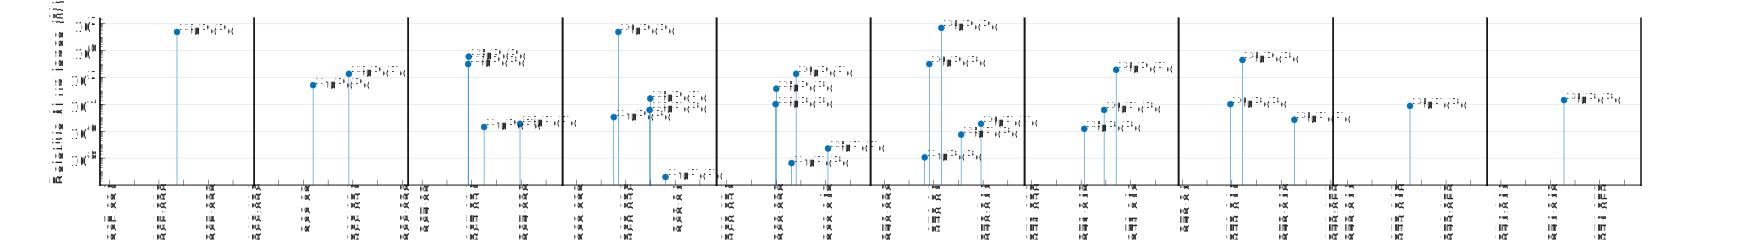
\includegraphics[keepaspectratio]{index_files/mediabag/figs/uranium_oxide_isotopologues.pdf}}

}

\caption{\label{fig-uranium_oxide_isotopologues}Uranium oxide (UO\(_2\))
isotopologues for a natural U sample with a \(^{233}\)U-\(^{236}\)U
tracer added. The \(^{238}\)U/\(^{236}\)U ratio is 0.5 for this sample,
and the tracer \(^{233}\)U/\(^{236}\)U is 1. Click to enlarge the
figure.}

\end{figure}%

\subsection{Energy, Electricity, and
Magnetism}\label{energy-electricity-and-magnetism}

To separate dissimilar objects like minerals or legos, one good strategy
is to place them all together and then sort through and choose different
elements from the pile. A chemical reaction might dissolve or
precipitate one element and leave another behind. However, isotopes of
the same element have nearly identical chemical behavior. Mass
spectrometers don't inspect and sort a stack of static individual atoms
like sorting legos, and they can't rely on chemical reactions to sort
isotopes.

Instead, mass spectrometers move the atoms by first ionizing them and
then manipulating the ions with electrical and magnetic forces. The
resulting kinetic changes in the isotopes' motion depend on their atomic
or molecular mass, which can be exploited to separate different
isotopes. Once separated, the streams of ions in motion must be measured
by sensitive electronic instruments. Here again, the ions' electrical
properties are important.

\subsubsection{Energy}\label{energy}

\begin{equation}\phantomsection\label{eq-kinetic_energy}{
KE = qV = \dfrac{1}{2}mv^2
}\end{equation}

\begin{Shaded}
\begin{Highlighting}[]
\ImportTok{import}\NormalTok{ numpy }\ImportTok{as}\NormalTok{ np}
\ImportTok{import}\NormalTok{ matplotlib.pyplot }\ImportTok{as}\NormalTok{ plt}

\NormalTok{kg\_per\_amu }\OperatorTok{=} \FloatTok{1.66e{-}27}
\NormalTok{mass\_amu }\OperatorTok{=} \DecValTok{238}
\NormalTok{mass\_kg }\OperatorTok{=}\NormalTok{ mass\_amu }\OperatorTok{*}\NormalTok{ kg\_per\_amu}
\NormalTok{velocity\_meters\_per\_second }\OperatorTok{=}\NormalTok{ np.linspace(}\DecValTok{0}\NormalTok{, }\DecValTok{2}\NormalTok{, }\DecValTok{100}\NormalTok{)}
\NormalTok{kinetic\_energy\_joule }\OperatorTok{=}\NormalTok{ mass\_kg }\OperatorTok{*}\NormalTok{ velocity\_meters\_per\_second }\OperatorTok{**} \DecValTok{2}

\NormalTok{fig, ax }\OperatorTok{=}\NormalTok{ plt.subplots()}

\NormalTok{ax.plot(velocity\_meters\_per\_second, kinetic\_energy\_joule)}

\NormalTok{ax.set\_xlabel(}\StringTok{\textquotesingle{}Veclocity (m/s)\textquotesingle{}}\NormalTok{)}
\NormalTok{ax.set\_ylabel(}\StringTok{\textquotesingle{}Kinetic Energy (J)\textquotesingle{}}\NormalTok{)}
\NormalTok{ax.set\_title(}\StringTok{\textquotesingle{}Stupid Plot\textquotesingle{}}\NormalTok{)}
\NormalTok{fig.tight\_layout}

\NormalTok{plt.show()}
\end{Highlighting}
\end{Shaded}

\begin{figure}[H]

\centering{

\pandocbounded{\includegraphics[keepaspectratio]{background_files/figure-pdf/fig-energy-output-1.pdf}}

}

\caption{\label{fig-energy}Kinetic energy as a function of velocity for
\(^{238}\)U}

\end{figure}%

\subsubsection{References}\label{references}

\phantomsection\label{refs}
\begin{CSLReferences}{0}{1}
\end{CSLReferences}

\bookmarksetup{startatroot}

\chapter{Overview}\label{overview}

\section{What is a Mass
Spectrometer?}\label{what-is-a-mass-spectrometer}

A mass spectrometer separates atoms by their atomic mass. Scientists
have long known how to separate different elements based on their
chemical properties. Thousands of years ago, metallic copper was first
smelted from copper ore, giving rise to the
\href{https://en.wikipedia.org/wiki/Chalcolithic}{Copper Age}. Modern
geochemical labs efficiently separate even very chemically similar
elements, such as the rare earth elements, via techniques like anion
exchange chromatography. These techniques separate one element from
another, like separating samarium (Sm) from neodymium (Nd).

Recall that the number of protons in an atom determines the number of
electrons that are needed to balance their charge. The number of
electrons in an atom determines its chemical behavior ---- whether and
how it makes chemical bonds with other atoms. But the nucleus of an atom
doesn't just contain protons, it also contains neutrons. Atoms with the
same number of protons but different numbers of neutrons are called
isotopes. Different isotopes of the same element behave in a chemically
similar manner: you can make CO\(_{2}\) with \(^{12}\)C, \(^{13}\)C, or
\(^{14}\)C.

The relative abundances of the isotopes of an element are key to a broad
array of geological processes, including the radioactivity used as a
clock in geochronology, geochemical processes that fractionate
radioactive parent isotopes from their radiogenic daughter products, and
temperature- and environment-dependent kinetic reaction rates. To
separate isotopes by their atomic mass, we need a mass spectrometer.

Separating atoms by their atomic mass is usually accomplished by first
ionizing the atoms, for instance by stripping an electron off to create
an ion with a \(+1\) positive charge. The ions can then be separated
according to their mass-to-charge ratio, often denoted \(m/z\).

This section describes the physical and chemical principles of mass
spectrometry.

\subsection{Table of Contents}\label{table-of-contents}

\begin{enumerate}
\def\labelenumi{\arabic{enumi}.}
\tightlist
\item
  \href{background.qmd}{Physics and Chemistry Refresher}
\end{enumerate}

\subsection{Equations to memorize}\label{equations-to-memorize}

Equation Equation~\ref{eq-kinetic_energy}

\bookmarksetup{startatroot}

\chapter{Ion Sources}\label{ion-sources}




\end{document}
